% Chapter 1

\chapter{State of the art}

\label{State of the art}

\cite{survey1}
\section{Botnets}
\cite{survey2}
As stated in the introduction botnets are an important problem for anyone involved somehow with the internet. They can result in great economic damage.
\cite{report1} 
Especially with their continuous improvement to become more resilient and powerful which makes them an even more important threat.\\\\
\cite{pheonix} 
Botnets can become very lucrative and can infect very large amount of devices resulting in scary tool. Here are some examples of the magnitude they can reach: \textbf{Flashback} with 600k compromised targets, \textbf{Grum} with 840k compromised devices and sending 40 Billion spam emails per month, \textbf{TDL-4} with 4.5 Million victims in first the 3 months and \textbf{Gameover ZeuS} with 1 Million infections, because of its resilience mechanisms this botnet was one of the hardest to take down.\\\\
\cite{survey2}
The reason botnets are still an ongoing research topic is that there isn't a complete solution for their detection and mitigation. Researchers and organisations have to keep working to keep updated with all the new flavors criminals bring to the market.
\subsection{Definition}
% WHAT IS A BOTNET?
\cite{memoire1}
\cite{detection1}
\paragraph{What is a botnet?} A botnet is a network of infected machines with programs called bots, these bots owned and controlled by a remote attacker called the botmaster. Users get infected via the same vector attacks used by malware, email attachment, malicious website, unaware download, etc. When bots usually infect these machines in stealthy manner, staying as unnoticeable as possible. The control of such bots is done through the Command and Control (CnC) server. The CnC server allows the master to issue commands to and receives responses from individual bots or aggregations of bots. These exchanges are done to update the software of the malware, execute attacks, exfiltrate data and more actions explained down below.
\cite{survey3}

%WHAT IS A BOT?
\cite{honeynet}
\paragraph{What is a bot?} Bots are small programs allowing to remotely control and perform commands on computers. They are the foundation of botnets. The paper presented by the SANS institute considers two types of bots. Bots used to perpetuate attacks, bots used for their content and both. \cite{tracking}
\cite{bot-com}
A clear distinction between a bot agent and a common piece of malware lies within a bot's ability to communicate with a Command-and-Control (CnC) infrastructure. CnC allows a bot agent to receive new instructions and malicious capabilities, as dictated by a remote criminal entity. This compromised host then can be used as an unwilling participant in Internet crime as soon as it is linked into a botnet via that same CnC.\\
These programs are embedded with port scanning, vulnerability scanning, exploitation kits and payloads that allow them to spread the botnet and infect their victims.\\
There are many different families of bots, some very modular such as the Agobot others less complete but easier to use such as the SDBot family. Bots families are also classified depending on the channel type and attack type, for example GT-Bots are a IRC bots but there are a lot of different protocols exploited as botnets channels. These 3 families are the most often found. Lesser usual ones have specific functions or plugins to fill in the gaps left by developers to customize the bots, a good examples would be the Dataspy Network X bots. There are very small bots such as the Q8 Bots and Perl-based bots that still allow for a large range of commands and attacks. Finally some bots are composed of a single file like Kaiten bot which makes it very easy to upload to compromised machines.

%WHY BOTS PROVIDE EVEN MORE POWERFULL ATTACKS
\cite{survey4}
\paragraph{Why do botnets provide more powerful attacks?} Botnets give the control to the botmaster of two critical resources: CPU (processing power) and IP addresses (anonymity). Even if the use of CPU stays low on the infected machines, the aggregate of bots can provide power equivalent to supercomputers with the additional perk of executing traffic from different addresses instead of a single IP.

% PURPOSE + CURRENT DANGERS
\paragraph{What is the purpose of botnets?} All these resources make botnets very powerful to execute network attacks. 
\cite{bot-intro}
Cybercriminals use botnets to execute a long list of malicious activities and structure related actions, we have listed some of these but any type of cyber attack can be uploaded to these bots and executed.
\cite{honeynet2}

% ADVANCES IN BOTNETS
\cite{survey5}
\paragraph{What are the advances in botnets?} Another reason botnets are a big threat is that criminals have started to provide botnets as a Service (BaaS) which are considered a big part of the botnet economy. This popularized botnets are sold to anyone, this has made them an even bigger threat that they already were.
This BaaS is possible with decentralized architectures that can subdivided into smaller botnets to sold and then reintegrated to the parent botnet after use.
\cite{tracking}

\cite{memoire1}
\paragraph{What types of actions are performed by botnets?} A victim host could be infected by targeting known vulnerability or by infected programs. When the victim is infected, the botnet will try to stay stealthy and with the exploit kit installed, it can do an extensive amount of damage. Here are some of the methods to control the infected hosts.\\
This first list presents general use of botnets:
\begin{itemize}[noitemsep]
\item \textbf{Distributed Denial-of-Service Attacks} These attacks provoke a loss of service or connectivity. Used by hacktivist, criminals and companies to disturb targets for recognition, financial gain or advantage over competition respectively. (The services could be email servers, production servers, web servers but also any device reachable) \cite{honeynet2}
\item \textbf{Spam email campaigns} Bots are set as proxy nodes and then used to send large amounts of spam and phishing emails.\cite{honeynet2}
\item \textbf{Sniffing Traffic} Bots can start watching packets going through the compromised machine and start retrieving all valuable data passed in clear-text. Botnets have been even found to analyze others bots data and take over them if they belong to another botnet.
\item \textbf{Spying through Keylogging and file monitoring} Sniffing packets effectiveness is reduced by encrypted traffic. The solution is then to log the key strokes made by the users and retrieve sensitive information. This is done with a keylogger and filtering mechanism that targets specific use-cases (logins, password, ...) \cite{honeynet2}
\item \textbf{Spreading new malware} Botnets growth depends on their ability to expand. Compromised targets have an important task to keep spreading the botnet. They can download malware or send viruses via email, there are various methods depending of the botnet type and environment they want to spread the malware.\cite{honeynet2}
\item \textbf{Installing Advertisement Addons, Browser Helper Objects (BHOs) and Google AdSense abuse} These techniques are used for financial gain instead of disruption. These are based on websites using clicking based ads. The criminals set fake sites using advertising programs and then automate the bots to click on them to create revenue. Since the bots have different IPs it is very hard to detect the fraud.
\item \textbf{Manipulating online polls and games} These are known to exist to influence decisions and are expected to be further used in the future. This is also very effective since each bot uses different IP addresses.
\item \textbf{Mass identity theft} Stealing personal data such as mail accounts, intellectual property, military secrets, embarrassing information or bank credential. This is a combination of all of the above that allow to create campaigns based on that data collected. These campaigns make this stolen data effective through fake websites and spear phishing email attacks. \cite{tracking}
Regarding the personal information that can be found by bots on the home desktops, this paper explains that it must not be overlooked. The amount of data that can be contained in home applications can be very important(taxes, browsers, email contacts. They warn of the sensitive information that is often stored on home computers related to their company. This could expose intellectual property that can be then sold by the criminals.
\item \textbf{Host illegal sites} Child pornography and black market sites are some examples.
\item \textbf{Computation for cryptanalysis} This is a less expected use of botnets, but these distributed supercomputers can be used for cryptanalysis purposes. Computing rainbow tables, cracking passwords, bruteforcing keys or mining crypto currencies. With the success of cryptocurrencies in the last 2 years, this type of use for botnets has increased. The latest example is the Smominru Monero mining botnet, mining around 9000 moneros worth at the time 3 million\$.
\cite{monero} \cite{tracking}
\end{itemize}
\cite{survey6}
This second list targets activities of bots on the compromised machines to take full control:
\begin{itemize}[noitemsep]
\item \textbf{Secure the system(close NetBIOS shares, RPCDCOM) to avoid infection by other criminals} This could also mean remove existing bots on the machine. Bots will make sure their host is properly hardened to avoid overtake.
\item \textbf{Redirect traffic for the botnet} Depending on the topology used, bots might be used as proxies to send commands, updates, data to the rest of the bots.
\item \textbf{Kill unwanted process running on the system} This joins the hardening objective. Bots want to take full control and make sure no process is limiting their actions (usually trying to stay stealthy while doing it).
\item \textbf{Test for virtual machines and/or debugger software} Part of the resilience of botnets resides in the obscurity of the mechanism they use. Honeypots will try to capture bots and do malware analysis to understand how they work. This tests will try to prevent this analysis to happen. (By deleting themselves or not executing in these environments)
\item \textbf{Add or delete auto-start applications} To stay resilient after reboot or even fresh installs, bots have mechanisms to stay persistent on the machine after those events.
\item \textbf{Run or terminate programs} This one is obvious but after exploiting the victim, their goal is to execute actions on the machine.
\item \textbf{Download and execute files} This allows them to update their software, download exploits and payloads. It can also be used to upload normal programs used for some of the tasks they want to execute.
\item \textbf{Perform address and port scan} Another important one to pivot inside networks and expand the botnet surface.
\item \textbf{Communicates with a handler or controller via public servers or other compromised systems} This is the  main channel communication with the botmaster.
\item \textbf{Data storage} One of the tactics used by botmasters to keep their anonymity is to use their botnet as a distributed database and saving the data obtained on the bots, this gives more distance with the stolen data.\cite{tracking} 
\end{itemize}

\subsection{Life cycle}
\paragraph{What are the steps that make up a botnet life cycle?} Life cycle execution might differ from one bot to another but they have generally a common structure. Here is the common structure presented in these studies: 
\cite{survey2}
\cite{survey7}
\cite{survey8}
\cite{survey9}
\begin{enumerate}
\item \textbf{Exploitation} The first phase is the infection of the host. The bots gets access to the victim host through different possible vectors (email attachment, vulnerability scanning and exploit, obtained credentials, malicious site, ...). The next step of this phase consists on uploading to the host the binary of the bot. 
\cite{bot-appr}
The bot connects to a server of the botmaster and downloads it. This step is very important for this thesis because it is the first DNS lookup the bot will perform and it has been noticed as the most consistent behavior of bots. This is where the bots are going to start to hide their DNS activity.
\cite{detection2}
\cite{detection3}
\cite{inside-bot}
\cite{detection4}
\item \textbf{Rallying} This is the phase where the bots will establish the link with the botmaster command and control servers (CnC), join the botnet and wait for instructions. When establishing the connection with the botmaster bots have to use stealth techniques to avoid getting discovered and more importantly revealing the CnC. These techniques will be discussed in the Misuses and abuses of DNS.
\cite{detection5}
\cite{detection6} 
\item \textbf{Attack/execution} From this point on the bot is ready to get the orders from the botmaster and start executing actions. This is where the different actions defined above are executed by the botnet.
\cite{survey10} 
\item \textbf{Update and maintenance}
This phase allows the botmaster to update periodically the software of the bots, new exploits, new attacks, the same way administrators patch their software. This final phase is a loop that goes back to the second phase where the bot contacts the CnC server to proceed to this binary upload and commands fetching. This is the second phase where the DNS request will use evasion techniques to stay hidden.
\cite{detection7}
\end{enumerate}
\subsection{The Channel}
\paragraph{What does it mean to join the botnet?} The bots will rarely directly connect to the CnC servers, they will go through proxies or peers bots, (structural nodes of the botnet) to obtain commands and updates. The knowledge of these nodes and the techniques used to communicate with them are the channel of a botnet.
\paragraph{What are the channels used by botnets?} The channel's resilience of a botnet is critical to ensure good communication with the CnC server. It is also a critical component because its failure is usually the end of the botnet's life. There are multiple ways of securing and hiding their communication channel: tunneling through protocols, encryption, DNS evasion techniques.
\cite{bot-intro}
The typical protocols that are used by bots to reach their CnC are these: IRC, HTTP, HTTPS, DNS, MAIL, SSH, etc. The use of different protocols implies there are a multiple botnet's communication topologies. The different topologies provide trade-offs in terms of bandwidth, rallying, stealth, ...

\paragraph{What are these different protocols ?}

\paragraph{What are the goals of these different channels?}
\cite{bot-com}
The main goal of the botnet channel is to provide a vector for bots to reach their CnC servers and maintain a connection with it. This is the only way the botmaster is able to keep control his botnet. This is why the means of communication are built around these main needs. If bots aren't able to reach the botnet or their CnC, they won't be able to update their software and receive commands.\\ 
Reaching and locating the CnC servers is the first challenge the channel needs to handle. Failing to do so will leave the bot unusable for the botmaster or left in a sleeping mode. In this state, the bot keeps on with the harvesting of the victim host and retry the missed CnC regularly. \\
The second challenge being its ability to maintain the channel. This is where resilient techniques have evolved to achieve this goal. These technologies will be detailed in the abuses of DNS section. CnC servers and their channels are really what differentiates botnets from other malware. 
%ABOVE 
\cite{cont-host} %file:///D:/CyberSecurityMaster/Master%20Thesis/papers/Botnet_general/botnet_review.pdf
	
\paragraph{How do botnets achieve such channels?}
\cite{detection5}
\cite{bot-threat}
To stay invisible and persistent channels have gone through different methods, here are the main ones: 
\begin{itemize}[noitemsep]
\item \textbf{Hardcoded IP}: The bot software has the IP address of the CnC server hardcoded somewhere in its binary. The server can be found through reverse engineering and the botnet could be stopped or suspended for a certain period.
\item \textbf{Dynamic DNS}: This is a solution to the hardcoded IPs. In this case the botnet will have multiple CnC servers migrating frequently on its will. In addition to using a dynamic list of servers, it uses dynamic DNS in order to avoid detection or suspension and keep the botnet portable. This allows the queries to be redirected if they were to fail. This behavior is known as herding, it provides mobility and stealth.
\item \textbf{Distributed DNS}: To avoid law, botmaster locate their DNS servers outside of the law's jurisdiction. Bots have the addresses of the DNS servers and contact them to resolve the IP address of the CnC servers.
\end{itemize}

\subsection{Topology}
\paragraph{How are the channels used ?}
Now that we know the purpose of channels and what they provide to botnets we are going to explore the different topologies used by botmasters using different channels and architectures.

\paragraph{What are the different topologies used by botnets?}

The differences between topologies are related to protocols of communication. Their structure will result as mentioned above in trade-offs for its different specifications.
\cite{survey6}
\cite{bot-intro}
As explained in this paper, there are two typical botnet topologies which all the other topologies are built on:
\begin{itemize}[noitemsep]
\item \textbf{Centralized}: This is the simplest structure. The CnC is the center of the architecture, responsible directly of the data and command exchanges with the bots. This central unit operates the whole botnet. The main advantages is speed and simplicity, this makes it easier to plan attacks and arrange the botnet. The big problem is that the CnC is the single point of failure of the architecture. If it goes down, the whole botnet is rendered ineffective. The main protocols used are IRC(Internet Relay Chat) and HTTP(Hyper Text Transfer Protocol, the protocol used to communicate between browsers and web servers). IRC is a client-server application for text messaging. The reason it is used as CnC servers is because it can set communications anonymously, between one and multiple users and is very easy to setup. Using the HTTP started because IRC channels were becoming to popular and IRC detection systems were being put in place. But this isn't the only reason: HTTP allows to hide CnC servers behind normal web traffic. This is perfect to be invisible to firewalls and IDS(Intrusion Detection Systems). One of the differences between both lies in how the information is passed: with IRC CnCs bots receive flows of commands from their botmaster, HTTP CnC wait for bots action to send them the commands.\cite{bot-com}
\item \textbf{Decentralized}: To avoid the single point of failure, botnet designers decided for a peer-to-peer (P2P) communication channel. This structure is much more resilient to detection and avoids the single point of failure. All bots are interconnected with each other and each one acts as client and server. New bots only need the addresses of some bots in the botnet to start communicating with the rest of the botnet. If parts of the botnet are suddenly offline or captured by authorities, the rest can still function normally and adapts rapidly to the situation.\cite{ict-11}
\end{itemize}
\paragraph{What are the metrics used to assess these architectures?}
The important metrics for a botnet are a combination of the above sections:
\begin{itemize}[noitemsep]
\item Resiliency: The ability to resist different events such as the loss of nodes in the botnet, loss of a CnC, blacklisting of domain names, federal investigations, etc.
\item Latency: Reliability on the transmission of messages. The botnet provides the bots a protocol to ensure the transmission of messages without.
\item Enumeration: Accurately predict the botnet's size.
\item Defense: protection mechanisms against reverse engineering, static and dynamic analysis, virtual environment execution.
\item Financially: Its potential to be partitioned and sold into sub-botnets. 
\end{itemize}

Botnets have followed the evolution of the defenses they were up against, for this is reason botnet operators have now a large choice of architectures when it comes to create one. Botnets topologies have been optimized to sustain most defenses and allow for large remote oversee. The choice of topology will be largely influenced by the business model the botnet operator has in mind.

\paragraph{What are the different topologies?}
CnC topologies encountered in the wild typically match one of the following types:
\begin{itemize}[noitemsep]
\item Star
\item Multi-server
\item Hierarchical
\item Random
\end{itemize}
%Modeling Botnets architectures:
%diurnal propagation model 
\cite{bot-prop}
%Super botnet model 
\cite{army-bot}
%Stochastic P2P model 
\cite{p2p-bot}
\cite{mobius}
%advanced P2P hybrid model 
\cite{hybrid}

\paragraph{Star}
\cite{bot-com}
The Star topology relies upon a single centralized CnC server to communicate with the rest of the botnet. Each bot agent is issued new instructions directly from the central CnC point. When a bot agent compromises a new victim, it is configured to reach its central CnC, where it will register itself as a botnet member and await for new instructions. The main problem with this topology is the single point of failure that constitutes the CnC server.
\cite{bot-intro}

\paragraph{Multi-server}
Multi-server is the logical follow up of the star topology, it is the combination of star CnC botnets joined together with the CnC servers connected to eachother. This is close to what is done in cluster database management with multiple servers deployed for load balancing and data replication. This ensures that if a CnC server is removed from the botnet, the other CnC servers will take its load and manage the bots that were connected to it. This topology is more complicated to setup, botmasters can even add a geographical component by having these CnC servers in the countries with bots deployed to improve speed and improve resistance to legal shutdowns.

\paragraph{Hierarchical}
Hierarchical topology is a tree based structure where any part of the tree can be used as a botnet on its own. In this topology, bots can proxy the CnC commands and instructions to the rest of the tree. Another interesting aspect of this architecture is that bots do not know the location of the rest of the botnet. They are aware of parts of it. This allows makes it harder to take down the botnet and allows to segment it for selling or leasing. The downside of it is the latency of the botnet introduced by its branching rendering certain attacks difficult.

\paragraph{Random - P2P}
This structure is decentralized and is composed of dynamic master-slaves or P2P relationships. Any bot can be used as CnC by the botmaster and relay them to the rest of the bots. To be told apart from the other traffic going through the botnet, traffic with commands will have a specific identification as a signature. This topology is very hard to take down because any node can be used as CnC, it also hard to hijack because there isn't a central structure and communications between nodes don't always use the same paths. The weakness of this topology is that it can reveal a lot of information about the botnet by simply monitoring a infected node and its communications with external hosts.

TODO
\paragraph{Hybrid}
\paragraph{P2P}

\paragraph{What design to pick ?} Here is a summary of the features taken into account when creating a botnet.\\
\begin{tabular}{|p{7cm}|p{7cm}|}
\hline
Pros & Cons \\
\hline
\multicolumn{2}{|c|}{Star}\\
\hline
\textbf{Speed of Control} &\textbf{ Single point of failure}\\
The direct communication between the CnC and the bots allows data to be transferred rapidly & CnC blocked or otherwise disabled results in the botnet rendered ineffective.\\
\hline
\multicolumn{2}{|c|}{Multi-server}\\
\hline
\textbf{No single point of failure} & \textbf{Requires advance planning}\\
Load balancing and replication prevents it from happening and maintains control of the botnet. & To achieve an infrastructure that is resilient and balanced such as multi-servers demands further preparation.\\
\textbf{Geographical optimization} & \\
Geographical location of severs speeds up communications between bots where the CnC servers are situated and help with law take downs.&\\
\hline
\multicolumn{2}{|c|}{Hierarchical}\\
\hline
\textbf{Re-sale} & \textbf{Command latency}\\
The botnet's owner can segment the sections of their botnet for lease or resale to other criminals. & Because commands must traverse
multiple communication branches within the botnet, there can be a high degree of latency with updated instructions being received by bot agents. This delay makes some forms of botnet attack and malicious operation difficult.\\
\textbf{Hidden topology} &\\
Compromised bots don't know the structure of the botnet therefore they are unable to leak much information.& \\
\hline
\multicolumn{2}{|c|}{Random}\\
\hline
\textbf{Highly resilient} & \textbf{Command latency}\\
The decentralized infrastructure and the many-to-many communication links between bot agents make it very resilient to shutdown. & The random nature of communication links between bots adds unpredictability to the system which can result in high levels of latency for some clusters of bot agents.\\
& \textbf{Enumeration}\\
& The analysis of a bot and its exchanges reveals a lot about the botnet structure and components.\\
\hline
\end{tabular}

IMAGE topologies (cf folder)

\newpage

\cite{phoenix}
\section{Uses and abuses of DNS protocol}
\cite{survey2}
The latest trend of botnet hide their channel through the DNS protocol. They use it to hinder their identification and rallying process.\\

\subsection{The DNS protocol}
\paragraph{What is the DNS protocol ?}
DNS stands for Domain Network System which main purpose is to "resolve" the IP address of a domain name (i.e. google.com).\\

\paragraph{How does the DNS work ?}
When an application tries to reach a certain domain, it send a DNS requests for the resolution of the domain name to the DNS server. \\
The server replies with a DNS response that contains the "answer" requested or additional information on how to obtain it.\\

\paragraph{What is the original purpose of DNS?}
The idea behind the protocol was to provide a human readable domain name to servers. That way humans could identify these domains and associate them with something concrete. The protocol simply looks for the server with the lookup table transforming them into machine readable addresses.
\cite{dns1}

\paragraph{Protocol example} to present usual behavior and better understand later, where the malicious actors abuse the protocol.\\
\cite{dns2}
When a client (user or device) tries to reach mail.google.com it sends a DNS request for that domain name from a \textbf{DNS client}.\\
The \textbf{DNS server} defined by the client receives the request and searches for it in its records. If it finds it then it sends the IP address to the DNS client. Otherwise, it will contact DNS name servers that could have the domain in their records following a specific logic in its search.\\
It will start by querying the \textbf{Root DNS servers} that will give it directions through the branches of the DNS tree hierarchy to the \textbf{Top Level Domains} DNS servers(TLD). It will first look for the TLDs resolving .com, then the name server that resolves google.com, down to the name server that will resolve mail.google.com to its IP address. The DNS server that received the first request will receive the response and send it to the client finally.\\
Finally, the client can now connect to the server using the resolved IP address.\\
TODO: DIAGRAM \cite{dns3}

\paragraph{Structure of the DNS packets?} To understand how the protocol is exploited we need to dive into the specifics of the packet structure.

\begin{verbatim}

			DNS packet
    +---------------------+
    |        Header       |
    +---------------------+
    |       Question      | the question for the name server
    +---------------------+
    |        Answer       | Ressource Records (RRs) answering the question
    +---------------------+
    |      Authority      | RRs pointing toward an authority
    +---------------------+
    |      Additional     | RRs holding additional information
    +---------------------+

\end{verbatim}
The format of a DNS message is the same for a request or a response but parts of the message will be filled differently. In the request, the client will fill the \textbf{Question section} with the information that needs to be resolved:
\begin{verbatim}
                                    1  1  1  1  1  1
      0  1  2  3  4  5  6  7  8  9  0  1  2  3  4  5
    +--+--+--+--+--+--+--+--+--+--+--+--+--+--+--+--+
    |                                               |
    /                     QNAME                     /
    /                                               /
    +--+--+--+--+--+--+--+--+--+--+--+--+--+--+--+--+
    |                     QTYPE                     |
    +--+--+--+--+--+--+--+--+--+--+--+--+--+--+--+--+
    |                     QCLASS                    |
    +--+--+--+--+--+--+--+--+--+--+--+--+--+--+--+--+
\end{verbatim}

\begin{tabular}{c|l}
value & explanation\\
\hline
q\_name  & Domain name requested (domain to be asked) \\
\hline
q\_type  & Type of RR record requested (A,AAAA,CNAME,MX,NS,PTR,...) \\
\hline
q\_class & Class of the request (often IN for internet) \\
\hline
\end{tabular}

\cite{dns4}
The server will respond by filling the \textbf{Answer section}: \\
\cite{dns5}
\begin{verbatim}
                                    1  1  1  1  1  1
      0  1  2  3  4  5  6  7  8  9  0  1  2  3  4  5
    +--+--+--+--+--+--+--+--+--+--+--+--+--+--+--+--+
    |                                               |
    /                                               /
    /                      NAME                     /
    |                                               |
    +--+--+--+--+--+--+--+--+--+--+--+--+--+--+--+--+
    |                      TYPE                     |
    +--+--+--+--+--+--+--+--+--+--+--+--+--+--+--+--+
    |                     CLASS                     |
    +--+--+--+--+--+--+--+--+--+--+--+--+--+--+--+--+
    |                      TTL                      |
    |                                               |
    +--+--+--+--+--+--+--+--+--+--+--+--+--+--+--+--+
    |                   RDLENGTH                    |
    +--+--+--+--+--+--+--+--+--+--+--+--+--+--+--+--|
    /                     RDATA                     /
    /                                               /
    +--+--+--+--+--+--+--+--+--+--+--+--+--+--+--+--+
\end{verbatim}

The important parts are the TTL (Time To Live) and the RDATA. TTL contains the span of time for which the Answer is valid, RDATA contains the answer to the RR requested.\\
\cite{dns6}
Here is a list of the main RR types and what they query.\\
\begin{itemize}[noitemsep]
\item \textbf{A or AAAA}: translation of a hostname into an IP address (IPv4 or IPv6).\\
\item \textbf{MX}: information regarding the mail servers of the domain queried (ex: DNS request for google.com with RR$=$MX could return mail.google.com) \\
\item \textbf{NS}: information about the DNS server used by that domain.\\
\item \textbf{TXT}: Text description of the domain queried.
\end{itemize}

\paragraph{Are there different methods to obtain the requested RR}
There are 2 methods of searching through the different DNS server from the \textbf{authoritative DNS} (DNS server assigned to or by the client DNS that will be queried first). It can be recursive or iterative. \textbf{Iterative mode} is an interaction between the authoritative DNS and all the other DNS servers where all request are initialized by it and all responses come back to it. \textbf{Recursive mode} is an interaction between DNS servers relaying the request and then coming back with the final answer. \\The Root DNS servers are always iterative, this has been set to avoid a DoS of those servers which could be caused if the were recursive. These servers are the backbone of the internet.

\subsection{Botnets abusing DNS}
%TODO: Present the different abuses of the DNS protocol to evade detection
%(use previous descriptions but revisit writing and add more visualization and explanations on how exactly it works. (it is important for future arguments regarding the evasion methods. We need to inform our reader to be able to convince him later of our arguments)

\paragraph{Why would botnets abuse the DNS protocol?}
DNS is a very attractive protocol for its versatility. Because DNS is used by all machines to locate other machines, DNS traffic is very normal in any network. Furthermore, the DNS protocol offers a lot of flexibility regarding its uses and this is where attackers have started using DNS for other purposes.
Looking up through DNS requests the CnC servers is an essential part in the lifecycle of a botnet. This has also made aware malicious actors that DNS traffic would be inspected to track them or detect them. To make the CnC lookup more resilient, botmasters searched multiple ways to lookup hostnames or play around them. This is where certain features of the DNS protocol became handy to fulfill that goal.
\paragraph{What features did they exploit ?}
Because of the growth of the internet, content providers have built complex infrastructures. Their goal is to sustain the load of the traffic and provide the best services. Some of the things implemented are load balancers, data fail-over, high availability through replication , security with end-to-end encryption, etc. To do so, they can use DNS features that allow to manage this type of architectures effectively. These features have inspired malicious actors with the following misuses: fast-flux, domain flux and DNS tunneling.

\subsubsection{Domain flux}
Domain-flux is a type of DNS feature that allows multiple domains to point towards the same IP address, making it hard to blacklist the domains related to the botnet. Bots are equipped with a special Domain Generation Algorithm (DGA). This is used to generate an ensemble of domains from which it will try to contact to received the next update. The idea behind generating such a big amount of domains is to register the domains that will come at a particular time and only register them exactly when they want to update the botnet and do it for a certain amount of time. The botmaster knows which domains are generated at a particular point in time since that is the seed of the algorithm and can register them before they are queried, that way they control when botnets can reach their CnC. This also improves the resilience of botnets infrastructure.

IMAGE: ADD picture explaining dga

\cite{bot-com}
\paragraph{There are the 2 techniques used to achieve domain fluxing}
\begin{itemize}[noitemsep]
\item \textbf{Domain Wildcarding} abuses the wilcarding capabilities of the DNS protocol. This can create rules that make all Fully Qualified Domain Names (FQDN) point to the same IP address. A rule defined by "*.example.com" would group all FQDN under that scope (mail.example.com, service.example.com, 123.example.com). DNS wildcarding is typical for phishing and spamming botnets. It allows to bypass some of the anti-spam defenses and even to use the wilcard argument as information to identify the different nodes (china01.example.com, china02.example.com).\cite{fqdn}
\item \textbf{Domain Generation Algorithms(DGA)} is the latest technology used by botnets for domain flux. It consists of algorithms that generate pseudo-random domain names based on a seed (this is the changing factor in the algorithm, ex: current time) chosen by the botmaster. This creates a list of FQDN that change constantly. Bots will try to reach all of the FQDN generated and when the botmaster wants to communicate with them, he will simply compute a couple of future FQDN and register them for his CnC servers to make them reachable by the bots and send the next instructions or updates. Since these domains only last a short amount of time, it becomes very complicated to block all of the possible generated domains through blacklisting or find the C2C servers.\\
In this github repository\cite{dga1}, they have compiled some examples of DGA used by famous botnets. As expected, the algorithms have 2 main functions, one that gets the seed (from input to the algorithm or using dynamic values such as date and time), the second is the domain generation, which will usually choose a TLD and then appends the result obtained from the random function with the dynamic seed.
\end{itemize}

\subsubsection{IP flux}
\paragraph{What is the concept of IP/Fast-flux networks?} IP-flux does the following: associate a certain number of IP addresses to a single FQDN. When sending a request to for the FQDN, one of these addresses is picked using the round-robin algorithm. This technique is normally used for load distribution, load balancing or fault-tolerance. All these addresses potentially host the identical servers, round-robin simply decides on the order it will present them when a request is made for the FQDN. The purpose was to enable IP-fluxing for Content Delivery Networks(CDN) to be able to point customers towards other nodes in the network to obtain the content sought.\cite{robin_dns} Round-robin divides time into small periods and presents equal blocks of these addresses in a circular order, it doesn't provide priority for any of the blocks of addresses or specific addresses.\cite{robin}\\

IMAGE: IP flux

\paragraph{How do botnets exploit this feature ?}
Fast-Flux is mostly used by botmasters to hide a malicious network behind a large amount of dynamic proxies(flux-agents).\cite{ff1} When a bot tries to connect with the CnC his request to the FQDN goes through a DNS server that returns one of these proxies which is picked from an immense list of rotating addresses. After that, the flux-agent relays the client's request to the mothership.\cite{wiki_ff} Behind the curtain of redirections created by the network of proxies, botmasters use it to distribute updates or host malicious content. They key elements for FFSN strength are very short TTLs and the round-robin answer from a large list of agents\cite{hybrid}\cite{tracking2}.
The Fast-flux Service Network (FFSN) motherships are the controlling parts of the networks. They are very similar to the command and a control (CnC) system found in conventional botnets but provide more features. It is observed that these nodes are managed as CDN servers with the same traits (high availability, load-balancing,...). To manage this complex network they collect all the information on the IP addresses assigned to the domain name and how those IP addresses (A and NS records) change over time.\cite{bot-com}\cite{detection3}

SOLVE biblio Issue

\paragraph{why is IP flux so effective?} Unfortunately, botnets use the DNS traffic as any other legitimate host, which makes differentiating the legitimate DNS traffic from the illegitimate, a very challenging problem [16]. Moreover, they use techniques to hide their communication with the bots to evade any deployed botnet detection processes [17]. The  botmasters use the DNS services to hide their command and control (CnC) IP address to make the botnet reliable and easy to migrate from server to another without being noticed.
\\
The power of FFSN is allowing one domain name to have an unlimited number of IP addresses. The IP addresses belonging to such a domain act as a proxy for any device attempting a connection with their respective CnC server. This process helps botnet controllers avoid detection and blacklisting. Attackers have developed better techniques utilizing IP-flux over time, here are the different categories:
\begin{itemize}[noitemsep]
\item \textbf{Single-flux}: Multiple IP addresses are assigned to the same domain (either CNAME or A records). The IP addresses of the bots are constantly registered and unregistered to the domain record. They have low TTL and most are proxies for master servers.\cite{wiki_ff}.
\item \textbf{NS flux}: Multiple NS records assigned to the same domain. This an additional layer of redirection, making the request go through multiples DNS servers before it reaches one that actually resolves the domain.)
\item \textbf{Double-flux}: Multiple name servers are assigned to the same domain and then use single-flux for the multiple IP addresses of the master. This provides a second layer of redundancy. This also means that the TTLs are short for the A records and the NS records too.
\end{itemize}

IMAGE replace these below by own pictures

Normal FF\cite{review1}\\
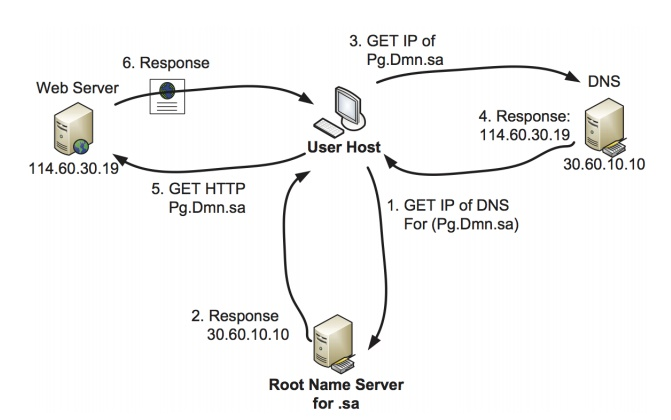
\includegraphics[scale=.7]{img/normal_FF.jpg}
single flux\\
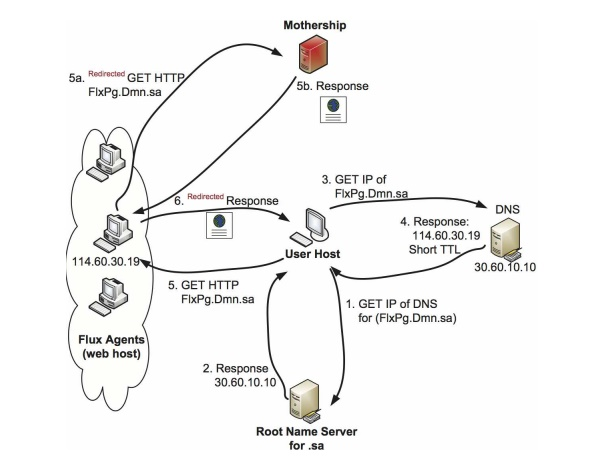
\includegraphics[scale=.7]{img/single_FF.jpg}
double flux\\
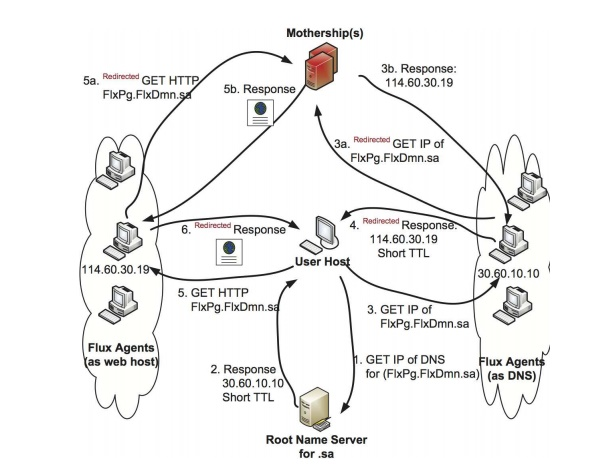
\includegraphics[scale=.7]{img/double_FF.jpg}


\subsubsection{DNS tunneling}
DNS tunneling implies the act of embedding other protocols or data through the DNS protocol. For example using the TXT  as q\_type or the subdomain itself to actually carry encoded data (i.e bWFsd2FyZQ.maliciousdomain.com, where bWFsd2FyZQ is encoded text). Usually, the payload will be fragmented to avoid unusual long domains or packets. This has been done to avoid restrictions but botnets also use it to hide malicious traffic or payloads. They can also use DNS tunneling to remain undetected while exfiltrating data. \cite{Botnet1}
What is positive about this abuse is that there are almost no legitimate reasons for this application, making obvious malicious behavior stands behind if this type of traffic is discovered.\cite{tunneling}

IMAGE tunneling (cf /img)


\subsubsection{Maybe Domain shadowing (need more research)}
\cite{review2}\cite{detection8}


\section{Machine learning approach}
We use machine learning in our thesis to create models around certain behaviors botnets show to helps us detect them from the legitimate traffic. The next sections will detail what machine learning is, how it works and its implementation in the thesis.
\subsection{Machine learning}
Machine learning (ML) is a mathematical study of algorithms and statistics that allow to learn and improve a certain task without being directly programmed. The goal is to improve the performance of specific tasks by building models of the problems. \cite{ml-def}

\subsection{Machine learning for botnet detection}
The goal of botnet detection is to distinguish which traffic is normal and which is malicious. We are interested in one of the tasks that machine learning algorithms excel at which is classification. After training the models, classification algorithms are able to predict the belonging of new data.

TODO: ADD DIAGRAM OF THE WORKFLOW

\subsection{Machine Learning workflow}
%https://cdn-images-1.medium.com/max/2000/1*KzmIUYPmxgEHhXX7SlbP4w.jpeg
Machine learning has a specific workflow that needs to be followed to obtain the best results: \cite{ml-workflow}: Gathering the data, feature extraction, choice of model, training and testing of the model, and assessment of the prediction capabilities of the model.

\subsubsection{Data gathering} The machine learning algorithms need to be fed data that has information about the problem. We need data that will be able to shape and create the model. In our case, we searched for captures of DNS traffic available publicly to study botnets, preferably labeled data as malicious or botnet. This labeling is essential for the learning stage. Another step which is important when creating the dataset is to balance it out correctly between the 2 labels. If there is an imbalance, the label with the greater presence in the dataset will influence the model excessively and poorly train it. The dataset research will be detailed in \label{datasetchapter}.

\subsubsection{Data pre-processing} 
Data pre-processing involves 2 processes: feature selection and feature extraction. The feature selection consists on deciding what elements of the data are relevant to create the model and feature extraction consists in cleaning the data and formatting it correctly to be ingested by the machine learning algorithms.\\\\

\paragraph{Feature selection} is an important step of the workflow. The choice of the data that will be ingested is crucial and directly connected to the results we will obtain. We chose to select features based on patterns or features based on data type. Pattern based means through statistical analysis of the data and using unsupervised learning algorithms to extract new tendencies from their results. The goal is to find patterns for each label, understand the underlying reason. Data type based means that we focus on the  specific features related to the traffic from the labeled data. Most of these features have been analysed by other researchers and will be based on the nature of the traffic coming from malicious and normal labels.\label{featureselectionlabel}

\paragraph{feature extraction} It is important to realize that algorithms are programs that only understand numerical data. The raw traffic captures can't directly be ingested by the algorithms, these can only digest 3 types of formats: numerical (300 seconds for the TTL of a record), categorical(DNS record types such as A, AAAA, TXT, CNAME, ...) and ordinal (short, medium, long). These formats can always be converted into numerical values which is the only thing algorithms can use. It is important to realize that only features from the data convertible into one of these formats will be able to be used. Format isn' the only thing that is important, with large datasets, we need to get rid of all the noise that they might contain as well as find missing data or inconsistency in parts of the traffic.
This section will be detailed in \label{featureextractionlabel}

\subparagraph{feature extraction techniques} To clean and extract the features from the raw data, there are common techniques used. The first is \textbf{conversion of data}, this consists in transforming the categorical and ordinal features into numerical ones (i.e [high, medium,low] would become [2,1,0]). The second consists in dealing with missing data by either removing it or using an average for that feature not to have it influence the other data for that feature. Thirdly, anomalies due to human errors for example need to be discovered and corrected. Finally, we normalize the features\cite{ml-norm} by dividing them by the maximum for that feature. The goal of the normalization is to avoid features unbalanced analysis by the algorithms(i.e. TTL is around $$[300-86400]$$ and number of resolved IPs $$[0-15]$$, TTL could have more weight in the algorithm due to the scale difference of the features). 

\subsubsection{How to chose the right algorithms?}
To answer this question we first need to learn which are the differences between the available algorithms and what they look to achieve: 

\paragraph{What are the different machine learning categories of algorithms?}
There are three mains categories of algorithms in machine learning based on their learning method: supervised learning, unsupervised learning and semi-supervised learning.
These categories are based on the training data given to the algorithms. \textbf{Supervised algorithms} are provided labeled data, they analyze the features and learn what characteristics are proper to each label. This is how the classifiers build models to predict the labels for new data.
\textbf{Unsupervised algorithms} use unlabeled data as input. This type of algorithm will group data based on similar values for different features.
Semi-supervised algorithms is the combination of both, where the training data is partially labeled. This is very useful for datasets where there is only partial labelisation available.
\\
TODO: ADD HERE CAPTION OF DIFFERENT CATEGORIES OF ALGORITHMS (supervised -> labeled(colors) then line between, unsupervised -> clusters, semi-super -> dunno yet)
\\
Now we need to decide what algorithm makes more sense to model the data in accordance to the problem that is being solved. We are trying to solve a detection problem. This falls into the typical classification problem as mentioned above where supervised algorithms prevail. To find the best algorithm to model the problem we will test out different algorithms and compare them under the same conditions.
\\
\\
Supervised algorithms have been chosen for the modeling part of the problem but unsupervised of algorithms will be used as well for the research of new features in the \textbf{features selection} step.

\subsubsection{Training and testing}
We now have a balanced and clean dataset with the chosen features. The way models are tested is by dividing a dataset into 2 sets, one for training and one for testing. In addition to this approach, it is combined with a second technique which is the 10-fold cross validation\cite{10-fold}. The training set will be used initially by the algorithm to learn and the testing set will be used to contrast the accuracy of the learning and create a feedback loop. The way datasets are divided into the 2 sets are up to us, the standard is 90-10 to train on a larger portion of the dataset but have a testing set big enough to include most of the variations. The cross validation technique will repeat the experiment changing the the training and testing sets for 10 loops equally and then average out the results, this allows to obtain more realistic results and unbiased by the randomness of sets chosen.

TODO:  A CAPTION EXPLAINING 10-fold

\subsubsection{Analysis of the model's prediction abilities}
Finally, we need metrics that will provide us information of the experiment. A very common way to do so is using the confusion matrix. This provides 4 main metrics that can then be exploited for more detailed information. There are other metrics \cite{ml-metrics} that can be introduced as well such as: 
\begin{enumerate}
\item Classification Accuracy.
\item Logarithmic Loss.
\item Area Under ROC Curve.
\item Classification Report.
\end{enumerate}
These metrics will allow us to understand what can be improved and the reason of the score obtained. From there we will adapt the features or the experiment to improve the results obtained. The goal is to reach the best results possible.

\subsection{How will machine learning be implemented for this Thesis?}
A big part of the work will be the feature selection. Going through the papers that have already done research on the subject, doing statistical analysis and using unsupervised learning to possibly extract more features and pick the ones we consider most effective. The algorithms used for detection as well as their parameters are an important part. Furthermore, the challenge in machine learning is to find the features with enough strength to create the model and the right settings for the classifiers so the fit the data correctly, it is very easy to fall in the over-fitting or under-fitting problem.

\subsection{Algorithm selection?}
Here we present the algorithms we will use.

TODO: CHECK HOW HE PRESENTS THE ALGORITHMS

\subsubsection{K-Nearest Neighbor}
kNN (k-Nearest Neighbor) is one of the simplest supervised machine learning algorithms.
The idea of kNN is that it will classify the new object based on its k nearest neighbors, where k is a
predefined positive integer [16]. kNN algorithm is comprehensively described in the following steps:
- Step 1: Determine the parameter value k.
- Step 2: Calculate the distance between the new object that needs to be classified with all objects
in the training dataset.
- Step 3: Arrange computed distances in the ascending order and identify k nearest neighbors with
the new object.
- Step 4: Take all the labels of the k neighbors selected above.
- Step 5: Based on the k labels that have been taken, the label that holds the majority will be
assigned to the new object.

\subsubsection{Decision Trees}
3.1.2.2. Decision tree
Decision tree is a prediction model that is a mapping from observations of a thing, or a
phenomenon to the conclusions about the objective value of things, or phenomena. Decision tree
creates models that allow the classification of an object by creating a set of decision rules. These rules
are extracted based on the set of characteristics of the training data. In a decision tree, leaves represent
classes and each child node in the tree and its branches represent a combination of features that
lead to classification. Thus, classifying an object will begin with checking the value of the root node,
and then continuing downward under the tree branches corresponding to those values. This process is
performed repeatedly for each node until it cannot go any further and touch the leaf node. For the best
model, the decision to select the root node and sub-node while building the decision tree is based on
the Information Gain (IG) and Gini Impurity measurements [16]. The decision tree algorithm used for
experiments in this paper is C4.5.

\subsubsection{Support Vector Machine}
\subsubsection{Logistic Regression}
\subsubsection{XGBoost}
\subsubsection{AdaBoost}
\subsubsection{Random forest}
%futureinternet-10-00043.pdf
3.1.2.3. Random forest
Random forest (RF) is a member of the chain of decision tree algorithms. The idea of this algorithm
is to create some decision trees. These decision trees will run and give independent results. The answer
predicted by the largest number of decisive trees will be chosen by the random forest [16]. To ensure
that the decision trees are not the same, random forest randomly selects a subset of the characteristics
of each node. The remaining parameters are used in the random forest as those in the decision trees.
Future Internet 2018, 10, 43 5 of 11

\subsubsection{Gaussian Naive Bayes}
3.1.2.4. Naïve Bayes
Naive Bayes is a conditional probability model based on the Bayes theorem [16]. In the
classification problem, the data includes: D is the set of training data that has been vectorized as
x = (x1, x2, ..., xn), Ci
is subclass i, with i = {1, 2, ..., m}. Assume that all properties are conditionally
independent of each pair together. According to Bayes theorem, we have:
P(Ci|X) = P(X|Ci)P(Ci)P(X)(1)
Based on the conditionally independent characteristic, we have:
P(X|Ci) = n k=1 P(xk|Ci) (2)
where, P(Ci|X) is the probability of class i given sample X, P(Ci) is the probability of class i and P(xk|Ci)
is the probability of the kth property that has the value of xk given X in class i.
\subsubsection{Neural Networks}

\section{Botnet detection related papers}
\subsection{classification of botnet research and detection}
In this section, we are going to present the current state of the botnet detection taxonomy, show the weaknesses and strengths of each method and end with the current state of the art of the research on passive traffic analysis for botnet detection which is the method this thesis is dedicated to.\\

\subsubsection{Taxonomy of Botnets}

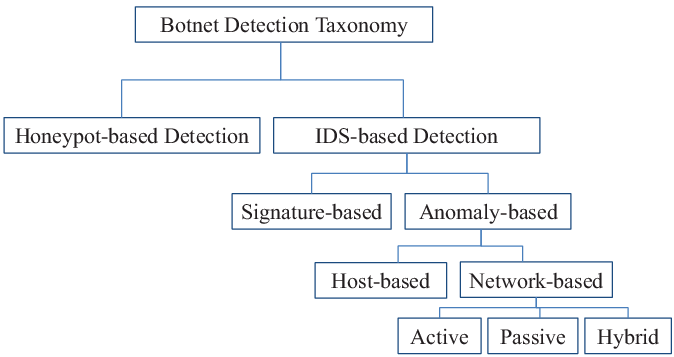
\includegraphics[scale=.8]{img/Botnet-detection-taxonomy.png}
%%%% SYSTEMS
\paragraph{Detection systems}In a recent survey\cite{survey1} of the state of the art regarding Botnet detection based on DNS traffic analysis\cite{survey}, they present a taxonomy of botnet detection techniques. As we can see on the figure (botnet\_detection\_taxonomy)there are 2 type of systems used for detection: Honeypots and IDS. Honeypots aim at creating an environment specially forged to attract malicious traffic and extract information out of the behavior of the malicious actor on the host. IDS aim at analyzing the network and alert the security analysts of any malicious/suspicious traffic. IDS are divided into 2 techniques. An older one based on signatures and newer one based on abnormal behavior.\\\\
%%%% IDS SIGNATURE-BASED
\paragraph{A legacy problem} A big trend among companies for a long time was a signature-based detection in their Intrusion Detection Systems ( IDS )\cite{bot-ml}. However, these signatures have shown to be ineffective against bots that are constantly getting updated with new code and evasion techniques. Furthermore, they are ineffective against any new type of emerging botnet. Signature-based detection is great for known botnets but remains weak to any new ones\cite{snort}. The recent introduction of other methods have been mostly motivated by the goal to solve this issue.
\\\\
%%%% NETWORK-BASED
\paragraph{Where are botnets detected?} In the anomaly detection technique, we have different locations that researchers have found relevant data. Directly on the host affected and throughout the network the host belongs to.
3 types of behaviors observed from the bots\cite{bot-threat1}:
\begin{itemize}
\item \textbf{network based behavior}: observable network traffic between botmaster and bots, it is used to detect individual bots and their CnC server. 
\item \textbf{host based behavior}: observable activity on the hosts infected by the botnets. 
\item \textbf{global correlated behavior}: global behavior characteristics, structure will be similar to current structures; same for all mechanisms
\end{itemize}
%%%% PASSIVE APPROACH
\paragraph{What are the types of approaches for detection?}
They are classified into 2 categories, passive and active detection\cite{detection9}. \textbf{Passive detection} consists gathering data through monitoring logs. Activity on the network is tracked without interfering with it, also making it harder for botmasters to notice it. This method is limited in the amount of data it can gather. Some examples of this approach: deep packet inspection through IDS, flow records analysis for traffic flow pattern identification, DNS monitoring, spam records analysis for botnet correlation, application log files analysis. \textbf{Active detection} differs from the passive approach by interacting directly with the information it observes. Because of the changes it may introduce, this approaches can be detected by the botmaster that might change the behavior of the botnet or add elements of evasion. There are 2 main examples: Sinkholing, this consists in redirecting the traffic of the botnet to a controlled machine to cut off CnC, and infiltration, which tries to wiretap or take control over the botnet from the inside by reverse engineering the malicious code and traffic. Other examples of active detection: FFSN tracking, IRC traffic analysis, peer-to-peer networks enumeration.
\\\\
This taxonomy applies to all botnets detection using different protocols. 
Let us now analyze the particularities the passive traffic analysis of the DNS protocol approach. The interest to study this part of the taxonomy comes from the progress it has shown and the large amount of possibilities around those techniques.

\subsubsection{Passive DNS detection Techniques}

%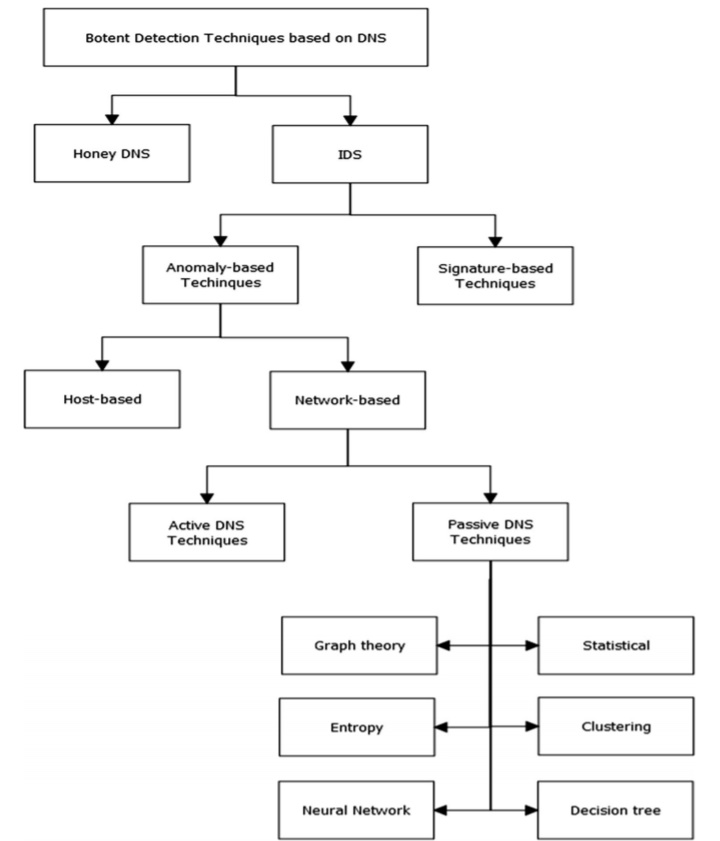
\includegraphics[scale=.8]{img/botnet_detection_techniques.jpg}
%%%% DNS taxonomy
%In a recent survey of the state of the art regarding botnet detection based on DNS traffic analysis\cite{survey}, they present a classification of botnet detection techniques via DNS \cite{survey1}. The newer techniques emerged to detect unknown botnets and to respond to the new type of evasions that followed. Botnets have become a lot more resilient and stealthy. It has pushed the research to focus on features that would allow to distinguish between benign and malicious traffic. Techniques capable of detecting new bots are divided into 2 sections: host-based and network-based. This means anomalies focusing on a single host or the traffic of a network. The host-based research focused on detecting bots in single hosts by monitoring local processes and kernel level routines.(TODO BotSwat) The problem of these propositions were the inability to scale them, we would need large monitoring system on each host with complex capabilities to communicate with each other and do correlation(TODO EFFORT framework). This is what the second section aims to solve by monitoring networks. This activity can be done passively by simply collecting the traffic and analysing it (passive monitoring). It can also been done actively by injecting packets into the network forged to make the bots react, and then analyse the network response. \\
%TODO: The part that our study focus on because "explain a valid reason for this part having more weight then the other ones, explain that our study could be a model combining different steps of the classification."

\paragraph{What are the different passive detection methods?}
With the logs or packets captured, researchers have proposed different approaches to utilize them, most of the techniques involve a statistical analysis or the use of machine learning algorithms others have opted for detection through visual representations. 
\\\\
The reason we have decided to focus on the machine learning approach as mentioned in the introduction is to develop our machine learning experience and methodology but also because regarding botnet detection it has shown to be the most effective method, achieving better scores then the other techniques in the taxonomy.
\\
In the machine learning realm, these are some of the techniques used: clustering, tree classification, neural networks, entropy, statistical,..
\\\\
As explained in the abuses of the DNS protocol, a new type of detection techniques have appeared that aim at finding bots evading the more usual detection techniques. 

\subsection{research review}
Now that we know the detection techniques used against botnets for different topologies and evading techniques. Here is a survey of the research papers that have proposed different techniques to detect botnets using these different evasion techniques presented in the abuse section of the DNS chapter.
%%%%%%%% TO BE REVIEWED
Since the end goal is to find the best features for an all-in solution, we have structured the current state of research as follows: 
First we will present the current all-in solutions that exist, the features they extract and what model they have created. 
Secondly, to achieve our goal towards improving these solutions, the objective is to find better features and better models. We will present studies focused on single detection models that cover the field of detection through passive DNS analysis. For each study we will list the features proposed, understand their purpose.\\
%%%%%%%%%%%%%%%%%%%%%%

========================================================================================
%CHECK PAPERS and EXTRACT VALUE

%Honeynet: capture and analyze Pros: Easy to build, low ressources requirements Cons: Hard to scale, limited interactions + can be reverted by hackers to learn new evasion techniques. \cite{bot-ml}
%IDS: monitor and look for signs 2 types\cite{survey11}: signature or anomaly based through DNS analysis(most promising) \cite{detection10}
%Anomaly detection approaches that work:  DNS Blacklist (for malware, botnets and spambots) \cite{dnsbl} and detect botnets when they try to communicate with their CnC:
%- NXDomains \cite{detection11}
%- recursive DNS queries detecting botnet related services \cite{detection12}
%- DGA 
%	1) Main DGA \cite{dga2}
%	2) Decision tree + Bayes for DGA classification \cite{detection13} 
%- Kopis = high level DNS query analysis (upper hierarchy)\cite{detection14}
%- Exposure \cite{passive-dns}
%- graph analysis \cite{dns-fail}
%- reputation system \cite{reputation} 

%Finally explain the different passive approaches: 
%Explain that these passive detection can also be divided into specific counters for certain evasion systems such as DF, FF, tunneling. Or be put together in an all-in solution to detect botnets independently of the evasion technique used.




\subsection{related papers}

%%%%% find where it belong


%TODO: check that paper again\cite{detection5} 
%"DNS Traffic Botmaster use DNS rallying to make their botnets invisible and portable. Choi et al. [20] proposed a botnet detection mechanism by monitoring their DNS traffic. Bots use DNS queries either to connect or to migrate to another CnC server. The DNS traffic has a unique feature that they define as group activity. Bots can be detected by using the group activity property of botnet DNS traffic while bots are connecting to their server or migrating to another server. There are three factors that help in distinguishing botnet DNS queries from legitimate DNS queries [20]; 
%(1) queries to CnC servers come only from botnet members (fixed IP address space size), 
%(2) botnet members migrate and act at the same time, which leads to temporary and synchronized DNS queries, 
%(3) botnets usually use DynamicDNS (DDNS) for CnC servers. 
%For a botmaster to keep its bots hidden and portable, he relies on DNS to rally infected hosts. In botnets, DNS queries can appear for many reasons. They appear during rallying process after infection, during malicious activities like spam or DoS attacks, during CnC server migration, during CnC server IP address change, or after CnC server or network link failure. Based on the aforementioned five situations of DNS query used in botnets, the authors have developed a Botnet DNS Q Detection algorithms, which distinguishes the botnet. This algorithm starts by building a database for DNS queries comprised of the source IP address, domain name and timestamp. Then, they group DNS query data using the domain name and timestamp field. After that, they remove redundant DNS queries. Finally, botnet DNS queries are detected using a numerically computed some similarity factor [20] This algorithm cannot detect botnets migrating to another CnC server. Therefore, they developed a Migrating Botnet Detection algorithm by modifying the botnet DNS query detection algorithm. Similarly, this algorithm starts by building a database for DNS queries comprised of the source IP address, domain name and timestamp. Then, it groups DNS query data using the domain name and timestamp field.
%After that, it removes redundant DNS queries. The next step will be to compare IP lists of different domain name with same size of IP list, because bots use two different domain names for the CnC server during migration [20]. These algorithms are protocol and structure independent and are capable of detecting unknown and encrypted botnets. However, these are not for real-time detections and have low accuracy for small networks. Furthermore, they are very sensitive to threshold values which need to be chosen very carefully to balance false positives and false negative rates.

\subsubsection{Domain-flux}
Domain-fluxing detection is mostly about analyzing domain names, here are the papers that attempt to do that with different metrics and features.\\
\\
Truong et al. \cite{dns-traffic} came up with an experiment allowing them to detect domains generated by humans or algorithms. This is the base-ground study of DGA detection. We use the features they propose to easily detect DGA domain names with the addition of later papers to distinguish between legitimate and malicious DGAs.\\
\\
Yadav et al. \cite{dga3} propose an unsupervised approach based on anomaly detection with a set of metrics analysing ngrams of the SLD. They use the Kullback-Liebler divergence measure with unigrams and bigrams, the Jaccard index between bigrams and the last feature and the Edit distance. These 3 features are used widely in the DGA detection research because of their efficiency, that is why we added them to our list of DGA features. \\
\\
Schiavoni et al. \cite{phoenix} go a step further then Truong et al. with their Pheonix project by improving the initial experiment with additional features to cluster groups of DGAs under the botnet families. Pheonix allows to associate new DGAs to certain botnets and follow the evolution of the different botnet families. We used the new features brought by Schiavoni et al. to improve our models for classification.\\
\\
Ahluwalia et al. \cite{dga} analyse the basic features that are common to most domain generated by DGA and provide advanced linguistic features to improve the results. The motivation for their work was due to recent botnets using shorter DGA lengths to blend with the other domains. They then propose 3 primitive features that capture linguistic and structural characteristics and 2 more advanced features that cover the shortcomings of the primitive ones. These features are simple but obtain really good results. They are an addition to our features for malicious DGA detection.\\
\\
%TODO: check if that paper is the same as used at the end?
Thomas et al. \cite{dga4} realized that during the domain generation process, most of the domains will not be up. This should result in a lot of NXDomain responses. Furthermore, the caching of NXDomains is limited which means that they cannot hide this traffic. Their contribution consists of a clustering technique based on domain names and request patterns; and similarity metrics for malicious domains detection. What can be retrieved from this study is the feature related to NXDomains and the clustering process for big datasets.

%In \cite{phoenix}, they explain the shortcomes of some of the other approaches. The study works in 2 phases: DGA discovery and DGA detection. In the discovery phase they apply the following filters that focus on linguistics: percentage of meaningful word in the domain name; popularity of the ngrams of the domain. They construct a base generated with the top 100.000 domains from Alexa. Then they define a distance (Mahalanobis distance) and thresholds(loose and stric ones) to determine when domains can be considered DGAs. They use known malicious domains to determine their thresholds. Afterwards they propose a sytem to cluster DGAs. They create a graph where each node is a domain and edges are created if both nodes resolve to similar IPs, the weight is proportional to the number of common resolved IPs. From all the "communities" discovered, they extract different common features to be reintroduced in the detection phase for each family of DGAs.
%%%%%%%%%%%%%%%%%%%%%%%%%%%%%%%%%%%%%%%%%%%
\subsubsection{Fast-flux}
%memoire
%%%%%%%%%%%%%%%%%%%%%%%%%%%%%%%%%%%%%%%%%%
The behavior of IP fluxing has been well analyzed by the community and most papers propose similar features to detect fast-flux. They often differ with different settings for their experiments. On the other hand, the big challenge for our thesis was to find the features that allowed us to find differences betweent malicious fast-flux networks(FFSN) and content delivery networks(CDNs). Both use fast-flux for different reasons making it hard to differentiate.\\
\\
The common features presented by  Salusky et al.\cite{honeynet}, Nazario et al.\cite{ff1}, Perdisci et al.\cite{ff2}, Holz et al.\cite{ff3} and Stalmans et al.\cite{ff_botconf} bring forward the features to detect fast-fluxing in general such as a large amount of unique A RRs for a domains, numerous unique NS for a domain and different Autonomous System (ASN) for the IPs linked to the same domain. \\
The next papers present additional features to distinguish detection specifically of the FFSN from the CDNs. \\
\\
Nazario et al. \cite{ff1} showed visually how the FF traffic features present themselves.
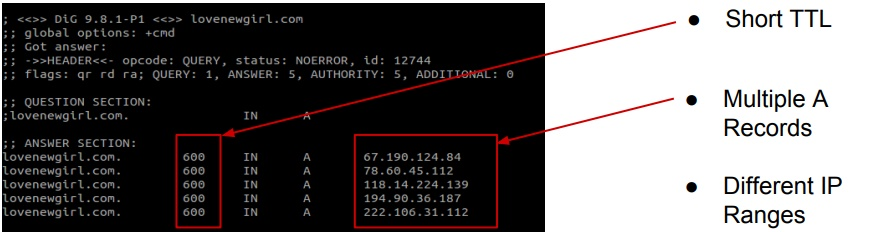
\includegraphics[scale=.7]{img/ff_features.jpg}\\
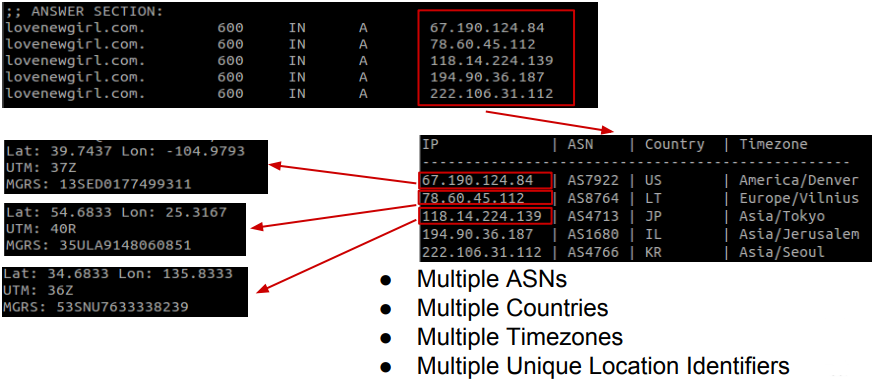
\includegraphics[scale=.6]{img/ff_features_2.png}
\\
Before the approach taken by \cite{ff2}, most of the detection was based on DNS Blacklisting (DNSBL), their new approach was a passive analysis of recursive DNS traffic. Recursive DNS  when your query is send to your DNS server, it starts by checking its cache and then will recursively ask other DNS servers until finding the address. Their purpose was to allow direct analysis of DNS requests and detect malicious ones. They want to improve the HoneyNet\cite{honeynet} features(short time-to-live (TTL), set of resolved IPs returned at each query changes rapidly, usually after every TTL, the overall set of resolved IPs obtained by querying the same domain name over time is often very large, the resolved IPs are scattered across many different networks)\\
They start by applying filters to cluster the different networks of FF using the list above. On these clusters they then applied statistical supervised algorithms to do the classification. They used a base of features provided by \cite{fluXOR} and added their own. \\It starts with the passive features: 
\\\\

They use these features on a Decision Tree classifier (efficient, easy to interpret and auto pruning of useless features) to classify malicious and legit FF networks.\\
\\
In the following paper\cite{ff3}, they propose some novel features compared to the other papers. To avoid redundancy, only the features not explored in previous papers will be detailed. In the paper they present the restrictions FFSNs face compared to CDNs: FFSN cannot choose the location which makes the IP address very scattered and no Uptime garantee. Possible distinctions: the lack of control results in number of unique A records returned different and the number of NS records in a single lookup (because the NS can be hosted inside the FFSN and return many NS records whereas legitimate CDNs return a very small set of NS records). The IP diversity restriction brings another feature which is the number of unique ASNs. Legitimate CDNs tend to return a single ASN for all their A records where FFSN are dispersed.\\
They decide not to include TTLs as a feature because both CDNs and FFSN have low TTLs. Finally,  they introduce functions of the different features above to classify FFSN and CDNs:fluxiness and flux-score\\
It could be argued that FFSN will try to mimic CDNs to have the same metrics, but as argued earlier, the metrics used take into account the restrictions FFSN have. The rest of the study approaches the detection of FFSN using the HTML content returned by the spam websites.\\

%Detection of Fast-flux Networks using Various DNS Feature Sets
This paper\cite{ff5} regroups the large majority of features encountered in the other papers accompanied with to some novel additions resulting a long list of 16 features.



%%%%%%%%%%%%%%%%%%%%%%%%%%%%%%%%%%%%%%%%%%%%%

\subsubsection{DNS tunneling}
%memoire
%%%%%%%%%%%%%%%%%%%%%%%%%%%%%%%%%%%%%%%%%%%%%%%
In \cite{tunn1}, use of TXT RR with segmented and encrypted data.
Rdata features: we look for the Shannon entropy of the strings. Measures the randomness of the string. Since encrypted data as a high level of entropy this is one of the things we'll be looking for. We are looking for "high byte entropy".Because of inherent reasons this entropy for a small string can't reach the max, we are looking at the "statistical byte entropy" instead.


They expect these behavioural communication features to be effective enough in order to extend a classifier based on the rdata features.
\\\\
In this paper\cite{tunn}, they propose a visual approach to detecting DNS tunneling, by plotting the following features, you can detect by "visual anomaly detection" the presence of DNS tunneling. 

\cite{dns-tun}

%%%%%%%%%%%%%%%%%%%%%%%%%%%%%%%%%%

\subsubsection{Behavioral}

\subsubsection{shadowing}

The first step in the research was to find the models that would be the current baseline for all-in solutions: because it is considered as the best all-in solution paper we could find, we are going to compare and extend the work of the EXPOSURE team.

\subsubsection{Combined approaches}

\paragraph{Exposure solution}
Bilge et al. \cite{exposure} created Exposure, a large-scale system that uses passive DNS monitoring of 15 features to detect malicious activity. The interesting parts of this paper were some of the unusual features proposed among the 4 categories of features presented and their pipeline for the project which we used for inspiration. What we look add to this paper is the low-scale part that is missing, some of the features are only available to ISPs and the idea is to scale it to any company with DNS monitoring capabilities.

\paragraph{Time-efficient local botnet infections}
Heuer et al. did a case study on local infections related to botnets\cite{localbotnet}. They propose a very large set of 24 features meant to detect botnets in networks . These features aim at the different evasion techniques that are used by botnets and the purpose is to be able to detect any form of Botnet in the network analysed.\\

\paragraph{Notos}
Antonakakis et al. \cite{dns-reputation} propose a different system called 'Notos' based on dynamic reputation od domain names. They studied the different aspects around the historical DNS data of domains that could be relevant to group domains based on their legitimacy. They use 3 categories of features: network, zone and evidence. They opted for a unsupervised approach using the clustering algorithm X-means. The purpose of this paper is to utilize some of the historical DNS features to be used in our all-in solution. Specifically, using some of the classes of domains defined by the authors as categorical features ( popular domains, common domains, Akamai domains,  CDN domains and dynamic DNS domains ).

\paragraph{DNS failures}
Yadav et al. \cite{dnsfailure} explore the detection possibilities in the DNS failed queries due to the fast fluxing behavior. Botnets are querying a large number of domains which are only up for specific amount of times, this results in NXDOMAIN responses from the DNS queries emitted, their research has tried to use this information to improve current detection systems.

A similar idea was proposed by Antonakakis et al. \cite{pleiades} creating Pleiades. First, following the same machine learning idea of Notos but applied to the DGA algorithms, meaning they applied the X-means clustering algorithm to DGA algorithms. Secondly, they used a boosted decision tree classification algorithm (Alternating Decision Tree) to test associations of an NXDomain's response to  DGAs. Finally, they created Hiddem Markov models for each of the DGAs domains to be able to classify the responses to a DGA directly. We'll use their work to improve the DGA features already gathered with the other papers.

%P1 Mean, median and standard deviation of 1-gram
%P2 Mean, median and standard deviation of 2-gram
%P3 Mean, median and standard deviation of 3-gram
%P4 Mean, median and standard deviation of 4-gram
%P5 Mean and standard deviation of entropy(d)
%P6 Mean and standard deviation of entropy(2LD)
%P7 Mean and standard deviation of entropy(3LD)
%P8 Mean, median, standard deviation and variance of domain name length
%P9 Mean, median, standard deviation and variance of # of domain levels
%P10 Number of distinct characters
%P11 Number of distinct TLD
%P12 Ratio of .com TLD
%P13 Ratio of other TLD
%P14 Mean, median and standard deviation of the occurrence frequency distribution for the different TLDs
%Table 8: Pleiades features


%- recursively collected historical dns information
%- domain name reputation (already tons of IP rep systems)
%- network and zone features capturing resource provisioning, usages, and management of domains.
%- model training through malicious and legitimate domain based on alexa, spam-trap, malware samples.
%- features: network/zone and evidence
%vocabulary: 
%d domain
%Zone(d) -> subdomains d
%D group of domains 
%A(D) -> IPs ever pointing to D
%a ip address
%BGP(a) -> all ips with bgp prefix of a
%AS(a) -> IPs in the Autonomous system of a

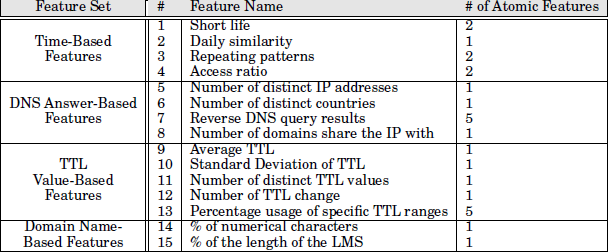
\includegraphics[scale=.3]{img/exposure_features.png}

